\begin{figure}[!ht]
    \centering
    \vspace{0.5cm}
    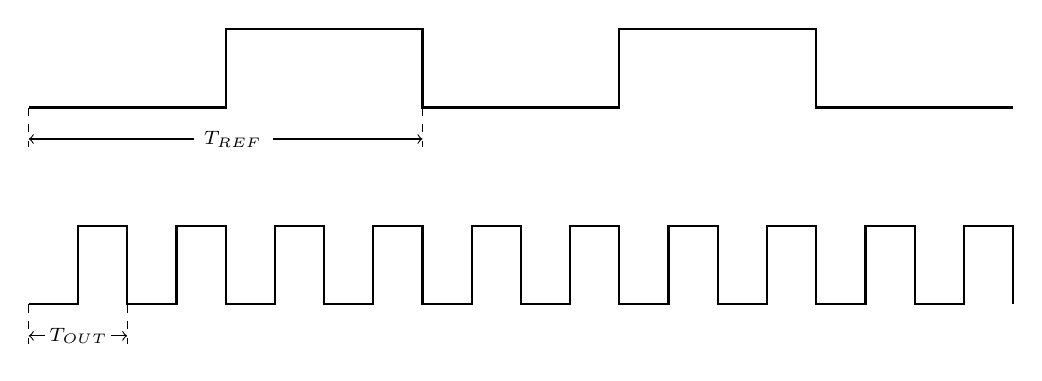
\begin{tikzpicture}

	\def \lref {0}
	\def \href {1}
	\def \lout {-2.5}
	\def \hout {-1.5}

        % Top signal: 2 periods of 10ns
        \draw[thick] (0,\lref) -- (2.5,\lref) -- (2.5,\href) -- (5,\href) -- (5,\lref) -- (7.5,\lref) -- (7.5,\href) -- (10,\href) -- (10,\lref) -- (12.5,\lref);
	%\node at (-0.5,0.5) {\scriptsize $f_\text{REF}$};

        \draw[<-] (0,-0.4) --++ (2.1,0) node[anchor=west]{\scriptsize $T_\text{REF}$};
	\draw[->] (3.1,-0.4) -- (5,-0.4);
    
	% Bottom signal: 8 periods of 2.5ns
        \draw[thick] (0,\lout) -- (0.625,\lout) -- (0.625,\hout) -- (1.25,\hout) -- (1.25,\lout) -- (1.875,\lout) -- (1.875,\hout) -- (2.5,\hout) -- (2.5,\lout) -- (3.125, \lout) -- (3.125,\hout) -- (3.75,\hout) -- (3.75,\lout) -- (4.375,\lout) -- (4.375,\hout) -- (5,\hout) -- (5,\lout) -- (5.625,\lout) -- (5.625,\hout) -- (6.25,\hout) -- (6.25,\lout) -- (6.875,\lout) -- (6.875,\hout) -- (7.5,\hout) -- (7.5,\lout) -- (8.125,\lout) -- (8.125,\hout) -- (8.75,\hout) -- (8.75,\lout) -- (9.375,\lout) -- (9.375,\hout) -- (10,\hout) -- (10,\lout) -- (10.625,\lout) -- (10.625,\hout) -- (11.25,\hout) -- (11.25,\lout) -- (11.875,\lout) -- (11.875,\hout) -- (12.5,\hout) -- (12.5,\lout);
	%\node at (-0.5,-1.5) {\scriptsize $f_\text{OUT}$};

        \draw[<-] (0,-2.9) --++ (0.2,0); 
	\draw (0,-2.9) ++ (0.63,0) node[]{\scriptsize $T_\text{OUT}$};
	\draw[->] (1.05,-2.9) -- (1.25,-2.9);

	\draw[dashed] (0,\lref) --++ (0,-0.5);
	\draw[dashed] (5,\lref) --++ (0,-0.5);
	\draw[dashed] (0,\lout) --++ (0,-0.5);
	\draw[dashed] (1.25,\lout) --++ (0,-0.5);
    
    \end{tikzpicture}
    %\vspace{0.5cm}
    \caption{Демонстарција рада синтетизатора фреквенције за FMUL=4.}
    \label{fig:fll:fref_fout}
\end{figure}
